%%%%%%%%%%%%%%%%%%%%%%%%%%%%%%%%%%%%%%%%%%%%%%%%%%%%%%%%%%%%%%%
%PANDOC SPECIFIC SHIT, TAKEN FROM ANOTHER TEMPLATE...

\documentclass[11pt,]{article}

%Deal with margins and other geometry stuff
\usepackage[margin = 1in]{geometry}
\usepackage{longtable}
\usepackage{booktabs}

% Need to include this for refs with Pandoc

%Some of this is math package stuff, but honestly i don't really get
%what most of it is doing
\usepackage{amssymb,amsmath}
\usepackage{ifxetex,ifluatex}
\usepackage{fixltx2e} % provides \textsubscript

%Numbered section spacing
\setcounter{secnumdepth}{0}

\usepackage{setspace}
\setstretch{1}

%For LIST (enumerate) spacing
\providecommand{\tightlist}{%
  \setlength{\itemsep}{0pt}\setlength{\parskip}{0pt}}

%%%%%%%%%%%%%%%%%%%%%%%%%%%%%%%%%%%%%%%%%%%%%%%%%%%%%%%%%%%%%%%%%%%
%% LUCY'S DOCUMENT PREAMBLE AND PACKAGES

\usepackage{pdflscape}
\usepackage{xcolor}

\usepackage{tcolorbox}
\newtcolorbox{blackbox}{
  colback=white,
  colframe=black,
  coltext=black,
  boxsep=5pt,
  arc=4pt}

%\usepackage[round]{natbib}
\usepackage[sectionbib, natbibapa]{apacite} 
\usepackage[hyphens]{url}

%Set paragraph indent and between paragraph spacing
\usepackage{parskip}
\setlength\parindent{0pt}
\setlength{\parskip}{0pt}

%Need all these for graphics and tables
\usepackage{subfig}
\usepackage{graphicx}
\usepackage{blindtext}
\usepackage{array}
\usepackage{float}

%Deal with titles and make them less stupid and ugly
\usepackage{titlesec}
\titleformat{\section}[block]{\bfseries\sc\filcenter}{}{1em}{}
%\titleformat{\section}[block]{\Large\bfseries\filcenter}{}{1em}{}
\titleformat{\subsection}[hang]{\bfseries}{}{1em}{}
\setcounter{secnumdepth}{0}

\usepackage[hyphens]{url}

%Bunch of hyperlink shit
\usepackage{hyperref}
\hypersetup{
    colorlinks=true,
    linkcolor=blue,
    filecolor=magenta,      
    urlcolor=cyan,
    citecolor = black
}


%Header and footer junk
\usepackage{fancyhdr}
\pagestyle{fancy}
\fancyhead[L,C]{}
\fancyhead[R]{\small{\textsc{L E Delaney} \hspace{3mm} \textit{Chapter
2: Single gene inheritance}}}
\fancyfoot[L]{\tiny{\textit{Version date: \today}}}
    \fancyfoot[R]{\thepage}
\fancyfoot[C]{}


%%%%%%%%%%%%%%%%%%%%%%%%%%%%%%%%%%%%%%%%%%%%%%%%%%%%%%%%%%%%%%%%%%%%%%%
%% START OF THE DOCUMENT BODY
\begin{document}

%%%%%% TITLE 
\begin{center}
\Large{\textsc{Chapter 2: Single gene
inheritance}}\\ \small{\textit{Problems 3, 40, 43, 46, 49, 18-19, 22,
27, 30, 13, 50, 53, 61}}\\
\vspace*{\baselineskip}
\end{center}

%%%%%%%%%%%%%% DOCUMENT BODY
\begin{blackbox}

\begin{enumerate}
\def\labelenumi{\arabic{enumi}.}
\setcounter{enumi}{2}
\tightlist
\item
  In Table 2-1, state the recessive phenotype in each of the seven
  cases.
\end{enumerate}

\begin{center}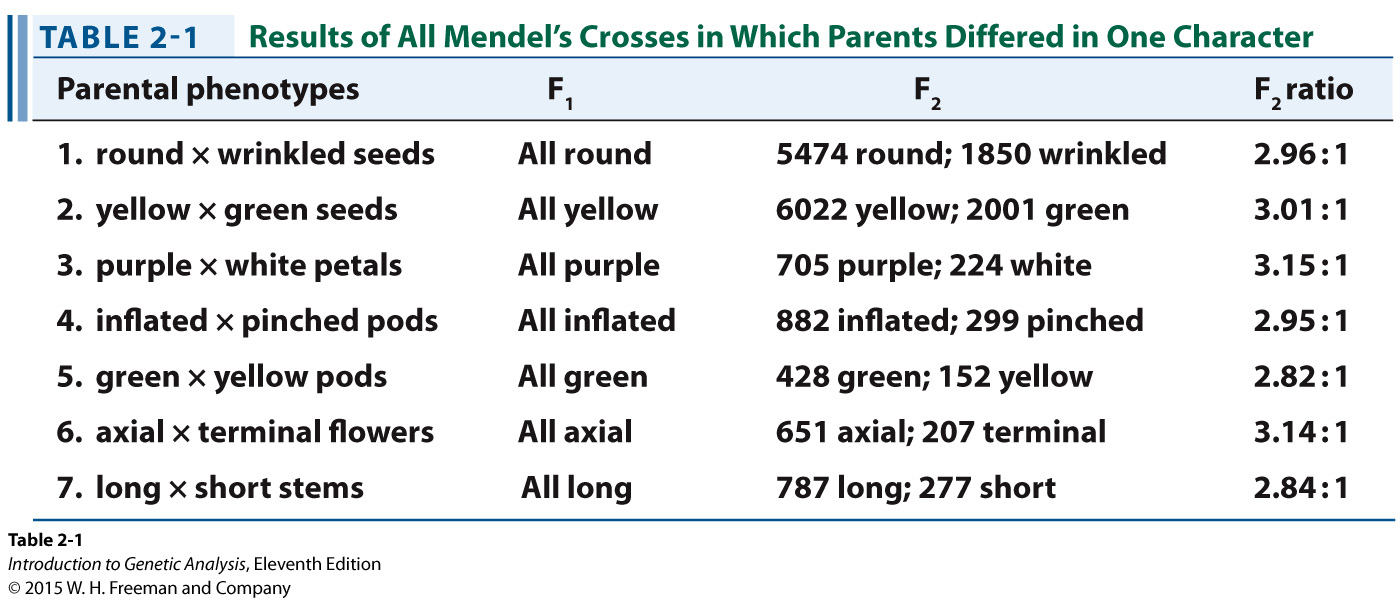
\includegraphics[width=0.35\linewidth,]{input/table_02_01} \end{center}

\textbf{Answer:}

wrinkled seeds; green seeds; white petals; pinched pods; yellow pods;
terminal flowers; short stems

\end{blackbox}

\begin{blackbox}

\begin{enumerate}
\def\labelenumi{\arabic{enumi}.}
\setcounter{enumi}{39}
\tightlist
\item
  In the plant \emph{Arabidopsis thaliana}, a geneticist is interested
  in the development of trichomes (small projections). A large screen
  turns up two mutant plants (A and B) that have no trichomes, and these
  mutants seem to be potentially useful in studying trichome
  development. (If they were determined by single-gene mutations, then
  finding the normal and abnormal functions of these genes would be
  instructive.) Each plant is crossed with wild type; in both cases, the
  next generation (F1) had normal trichomes. When F1 plants were selfed,
  the resulting F2's were as follows:
\end{enumerate}

\begin{itemize}
\tightlist
\item
  F2 from mutant A: 602 normal; 198 no trichomes
\item
  F2 from mutant B: 267 normal; 93 no trichomes
\end{itemize}

\begin{enumerate} 
 \item[a.]{ What do these results show? Include proposed genotypes of all plants in your answer. } 
 \item[b.]{ Under your explanation to part a, is it possible to confidently predict the F1 from crossing the original mutant A with the original mutant B?  } 
 \end{enumerate}

\textbf{Answer:}

The data indicates that each mutant is homozygous recessive for a
mutation that inhibits trichome development (aa). When crossed with
wild-type plants (AA), all F1 progeny were normal suggesting the
following cross:

\begin{longtable}[]{@{}lll@{}}
\toprule
\begin{minipage}[b]{0.09\columnwidth}\raggedright
\strut
\end{minipage} & \begin{minipage}[b]{0.11\columnwidth}\raggedright
a\strut
\end{minipage} & \begin{minipage}[b]{0.11\columnwidth}\raggedright
a\strut
\end{minipage}\tabularnewline
\midrule
\endhead
\begin{minipage}[t]{0.09\columnwidth}\raggedright
A\strut
\end{minipage} & \begin{minipage}[t]{0.11\columnwidth}\raggedright
Aa\strut
\end{minipage} & \begin{minipage}[t]{0.11\columnwidth}\raggedright
Aa\strut
\end{minipage}\tabularnewline
\begin{minipage}[t]{0.09\columnwidth}\raggedright
A\strut
\end{minipage} & \begin{minipage}[t]{0.11\columnwidth}\raggedright
Aa\strut
\end{minipage} & \begin{minipage}[t]{0.11\columnwidth}\raggedright
Aa\strut
\end{minipage}\tabularnewline
\bottomrule
\end{longtable}

Thus, the F1 progeny were all heterozygous and their offspring display
the expected 3:1 ratio from the following cross:

\begin{longtable}[]{@{}lll@{}}
\toprule
\begin{minipage}[b]{0.09\columnwidth}\raggedright
\strut
\end{minipage} & \begin{minipage}[b]{0.11\columnwidth}\raggedright
A\strut
\end{minipage} & \begin{minipage}[b]{0.11\columnwidth}\raggedright
a\strut
\end{minipage}\tabularnewline
\midrule
\endhead
\begin{minipage}[t]{0.09\columnwidth}\raggedright
A\strut
\end{minipage} & \begin{minipage}[t]{0.11\columnwidth}\raggedright
AA\strut
\end{minipage} & \begin{minipage}[t]{0.11\columnwidth}\raggedright
Aa\strut
\end{minipage}\tabularnewline
\begin{minipage}[t]{0.09\columnwidth}\raggedright
a\strut
\end{minipage} & \begin{minipage}[t]{0.11\columnwidth}\raggedright
Aa\strut
\end{minipage} & \begin{minipage}[t]{0.11\columnwidth}\raggedright
aa\strut
\end{minipage}\tabularnewline
\bottomrule
\end{longtable}

\end{blackbox}

\begin{blackbox}

\begin{enumerate}
\def\labelenumi{\arabic{enumi}.}
\setcounter{enumi}{42}
\tightlist
\item
  In the pedigree below, the black symbols represent individuals with a
  very rare blood disease. If you had no other information to go on,
  would you think it more likely that the disease was dominant or
  recessive? Give your reasons.
\end{enumerate}

\begin{center}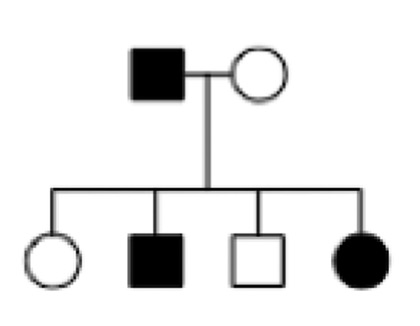
\includegraphics[width=0.35\linewidth,]{input/43pedigree} \end{center}

\textbf{Answer:}

If the disease were recessive, it would mean that the father has two
copies of the allele, and the mother has one. Otherwise, the children
could not be affected -- for them to have a recessive phenotype, they
must each inherit one allele from each parent! And yet, you are told
this disease is very rare. If it is dominant, it simply means the father
has one copy of the allele and he passed it to each of the parents.
Thus, the disease is likely dominant.

\end{blackbox}

\begin{blackbox}

\begin{enumerate}
\def\labelenumi{\arabic{enumi}.}
\setcounter{enumi}{45}
\tightlist
\item
  Suppose that a husband and wife are both heterozygous for a recessive
  allele for albinism. If they have dizygotic (two-egg) twins, what is
  the probability that both the twins will have the same phenotype for
  pigmentation?
\end{enumerate}

\textbf{Answer:}

Both parents are A/a. Both twins could be albino or both twins could be
normal (for probability calculations: and = multiply, or = add). The
probability of being normal is the probability of having one dominant
allele (A/--) -- \(\frac{3}{4}\). The probability of being albino is the
probability of having two recessive alleles (a/a) -- \(\frac{1}{4}\).

p(both normal) + p(both albino) =

p(first normal) \(\times\) p(second normal) + p(first albino) \(\times\)
p(second albino) =

\(\frac{3}{4} \times \frac{3}{4} + \frac{1}{4} \times \frac{1}{4} = \frac{9}{16} + \frac{1}{16} = \frac{5}{8}\)

\end{blackbox}

\begin{blackbox}

\begin{enumerate}
\def\labelenumi{\arabic{enumi}.}
\setcounter{enumi}{48}
\tightlist
\item
  In nature, the plant \emph{Plectritis congesta} is dimorphic for fruit
  shape; that is, individual plants bear either wingless or winged
  fruits. Plants were collected from nature before flowering and were
  crossed or selfed with the following results:
\end{enumerate}

\hfill\break

\begin{longtable}[]{@{}lll@{}}
\toprule
Pollination & Winged & Wingless\tabularnewline
\midrule
\endhead
Winged (selfed) & 91 & 1\tabularnewline
Winged (selfed) & 90 & 30\tabularnewline
Wingless (selfed) & 4 & 80\tabularnewline
Winged x wingless & 161 & 0\tabularnewline
Winged x wingless & 29 & 31\tabularnewline
Winged x wingless & 46 & 0\tabularnewline
Winged x winged & 44 & 0\tabularnewline
Winged x winged & 24 & 0\tabularnewline
\bottomrule
\end{longtable}

\textbf{Answer:}

\hfill\break

\begin{longtable}[]{@{}llll@{}}
\toprule
Pollination & Genotypes & Winged & Wingless\tabularnewline
\midrule
\endhead
Winged (selfed) & AA x A- & 91 & 1\tabularnewline
Winged (selfed) & Aa x Aa & 90 & 30\tabularnewline
Wingless (selfed) & aa x aa & 4 & 80\tabularnewline
Winged x wingless & AA x aa & 161 & 0\tabularnewline
Winged x wingless & Aa x aa & 29 & 31\tabularnewline
Winged x wingless & AA x aa & 46 & 0\tabularnewline
Winged x winged & AA x A- & 44 & 0\tabularnewline
Winged x winged & AA x A- & 24 & 0\tabularnewline
\bottomrule
\end{longtable}

The five unusual plants are most likely due either to human error in
classification or to contamination. Alternatively, they could result
from environmental effects on development. For example, too little water
may have prevented the seedpods from becoming winged, even though they
are genetically winged.

\end{blackbox}

\begin{blackbox}

\begin{enumerate}
\def\labelenumi{\arabic{enumi}.}
\setcounter{enumi}{17}
\tightlist
\item
  Name the key function of mitosis.
\end{enumerate}

\textbf{Answer:}

The key function of mitosis is to generate two daughter cells that are
genetically identical to the original parent cell.

\end{blackbox}

\begin{blackbox}

\begin{enumerate}
\def\labelenumi{\arabic{enumi}.}
\setcounter{enumi}{18}
\tightlist
\item
  Name two key functions of meiosis.
\end{enumerate}

\textbf{Answer:}

Two key functions of meiosis are to halve the DNA content and to
reshuffle the genetic content of the organism to generate genetic
diversity among the progeny.

\end{blackbox}

\begin{blackbox}

\begin{enumerate}
\def\labelenumi{\arabic{enumi}.}
\setcounter{enumi}{21}
\tightlist
\item
  In what ways does the second division of meiosis differ from mitosis?
\end{enumerate}

\textbf{Answer:}

As cells divide mitotically, each chromosome consists of identical
sister chromatids that are separated to form genetically identical
daughter cells. Although the second division of meiosis appears to be a
similar process, the ``sister'' chromatids are likely to be different.
Recombination during earlier meiotic stages has swapped regions of DNA
between sister and nonsister chromosomes such that the two daughter
cells of this division typically are not genetically identical.

\end{blackbox}

\begin{blackbox}

\begin{enumerate}
\def\labelenumi{\arabic{enumi}.}
\setcounter{enumi}{26}
\tightlist
\item
  If children obtain half their genes from one parent and half from the
  other parent, why aren't siblings identical?
\end{enumerate}

\textbf{Answer:}

Because the ``half'' inherited is very random, the chances of receiving
exactly the same half is vanishingly small. Ignoring recombination and
focusing just on which chromosomes are inherited from one parent, there
are \(22^3 = 8,388,608\) possible combinations!

\end{blackbox}

\begin{blackbox}

\begin{enumerate}
\def\labelenumi{\arabic{enumi}.}
\setcounter{enumi}{29}
\tightlist
\item
  Four of the following events are part of both meiosis and mitosis, but
  only one is meiotic. Which one? (1) chromatid formation, (2) spindle
  formation, (3) chromosome condensation, (4) chromo- some movement to
  poles, (5) synapsis
\end{enumerate}

\textbf{Answer:}

\begin{enumerate}
\def\labelenumi{(\arabic{enumi})}
\setcounter{enumi}{4}
\tightlist
\item
  synapsis (chromosome pairing)
\end{enumerate}

\end{blackbox}

\begin{blackbox}

\begin{enumerate}
\def\labelenumi{\arabic{enumi}.}
\setcounter{enumi}{12}
\tightlist
\item
  Could the pedigree in Figure 2-31 be explained as an autosomal
  dominant disorder? Explain.
\end{enumerate}

\begin{center}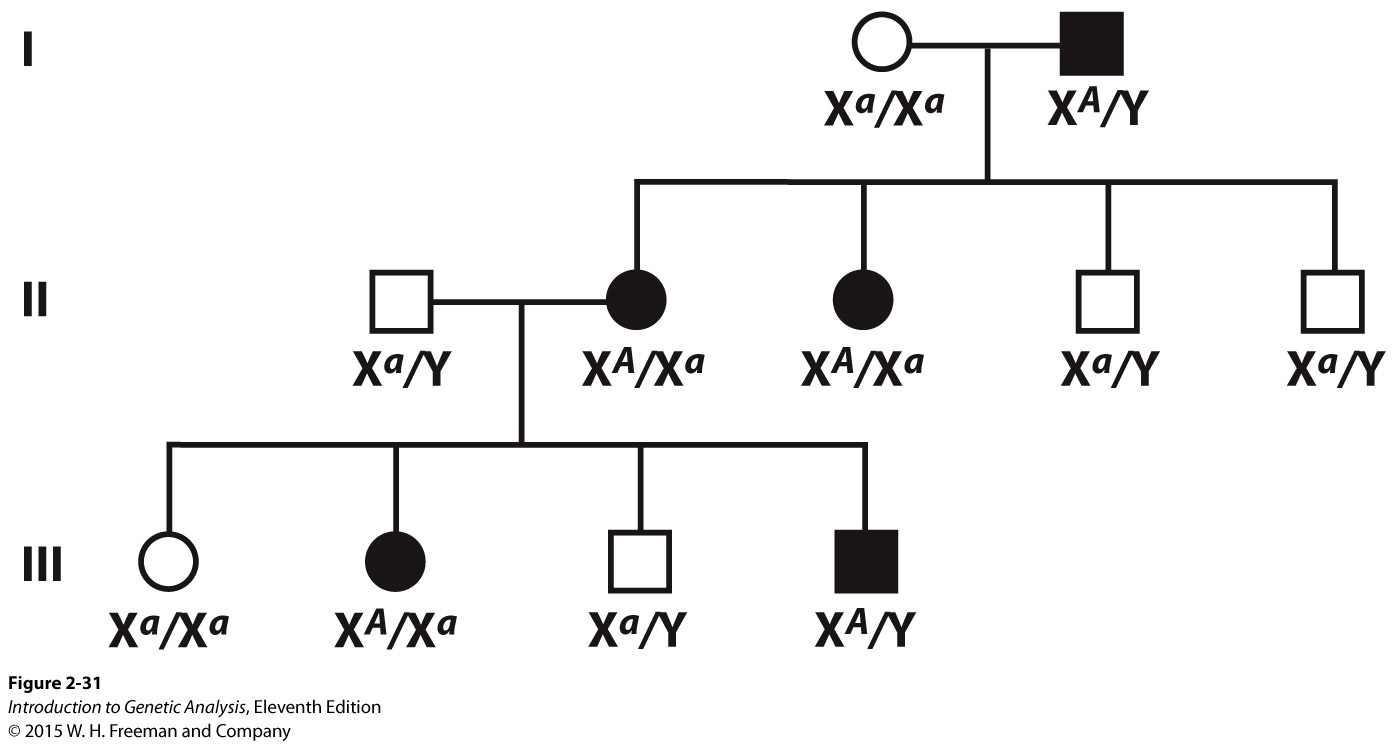
\includegraphics[width=0.35\linewidth,]{input/figure_02_31} \end{center}

\textbf{Answer:}

\end{blackbox}

\begin{blackbox}

\begin{enumerate}
\def\labelenumi{\arabic{enumi}.}
\setcounter{enumi}{49}
\tightlist
\item
  The accompanying pedigree is for a rare but relatively mild hereditary
  disorder of the skin.

  \begin{enumerate} 
   \item[a.]{ How is the disorder inherited? State reasons for your answer. } 
   \item[b.]{ Give genotypes for as many individuals in the pedigree as possible. (Invent your own defined allele symbols.) } 
   \item[c.]{ Consider the four unaffected children of parents III-4 and III-5. In all four-child progenies from parents of these genotypes, what proportion is expected to contain all unaffected children? } 
   \end{enumerate}
\end{enumerate}

\begin{center}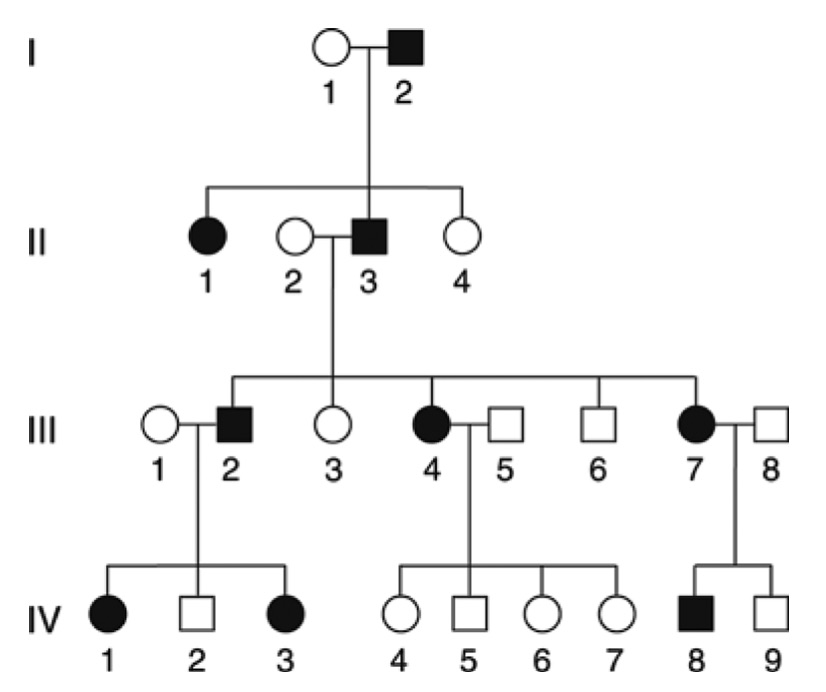
\includegraphics[width=0.35\linewidth,]{input/50pedigree} \end{center}

\textbf{Answer:}

\begin{enumerate} 
 \item[a.]{  } 
 \item[b.]{  } 
 \item[c.]{  } 
 \end{enumerate}

\end{blackbox}

\begin{blackbox}

\begin{enumerate}
\def\labelenumi{\arabic{enumi}.}
\setcounter{enumi}{52}
\tightlist
\item
  The following pedigree was obtained for a rare kidney disease.

  \begin{enumerate} 
   \item[a.]{ Deduce the inheritance of this condition, stating your reasons. } 
   \item[b.]{ If persons 1 and 2 marry, what is the probability that their first child will have the kidney disease? } 
   \end{enumerate}
\end{enumerate}

\begin{center}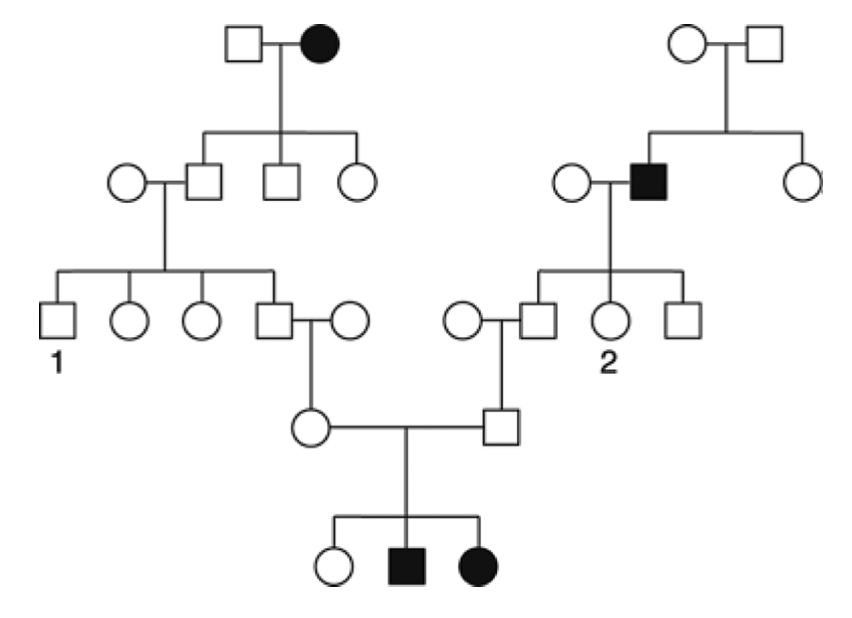
\includegraphics[width=0.35\linewidth,]{input/53pedigree} \end{center}

\textbf{Answer:}

\begin{enumerate} 
 \item[a.]{  } 
 \item[b.]{  } 
 \end{enumerate}

\end{blackbox}

\begin{blackbox}

\begin{enumerate}
\def\labelenumi{\arabic{enumi}.}
\setcounter{enumi}{60}
\tightlist
\item
  Duchenne muscular dystrophy is sex-linked and usually affects only
  males. Victims of the disease become progressively weaker, starting
  early in life.

  \begin{enumerate} 
   \item[a.]{ What is the probability that a woman whose brother has Duchenne’s disease will have an affected child? } 
   \item[b.]{ If your mother’s brother (your uncle) had Duchenne’s disease, what is the probability that you have received the allele? } 
   \item[c.]{ If your father’s brother had the disease, what is the probability that you have received the allele? } 
   \end{enumerate}
\end{enumerate}

\begin{center}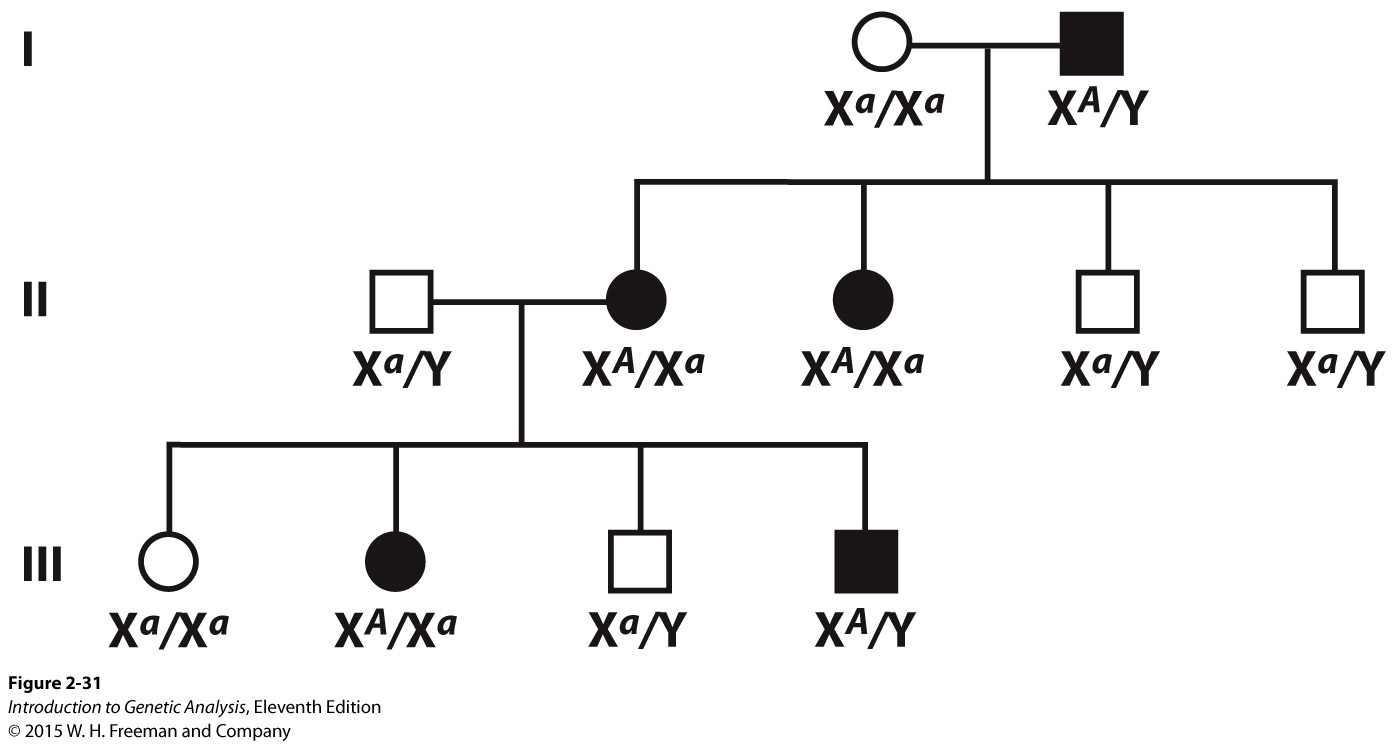
\includegraphics[width=0.35\linewidth,]{input/figure_02_31} \end{center}

\textbf{Answer:}

\begin{enumerate} 
 \item[a.]{  } 
 \item[b.]{  } 
 \item[c.]{  } 
 \end{enumerate}

\end{blackbox}

\end{document}


